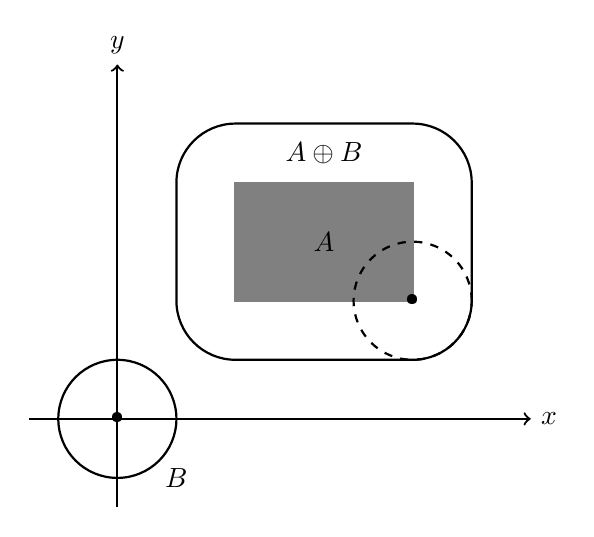
\begin{tikzpicture}[thick, scale=.75]
	% axis
	\draw[->] (-1.5, 0) -- (7, 0) node[right] {$x$};
	\draw[->] (0, -1.5) -- (0, 6) node[above] {$y$};
	
	% A
	\filldraw[gray] (2,2) rectangle (5,4);
	\node at (3.5, 3) {$A$};
	
	% Structuring element
	\draw (0, 0) node {\textbullet} ellipse (1 and 1);
	\draw[dashed] (5, 2) node {\textbullet} ellipse (1 and 1);
	\node at (1, -1) {$B$};
	
	% Dilation result
	\draw (6,4) arc (0:90:1) -- (2, 5) arc (90:180:1) -- (1, 2) arc (180:270:1) -- (5, 1) arc (270:360:1)  -- cycle;
	\node at (3.5, 4.5) {$A\oplus B$};
\end{tikzpicture}